\RequirePackage[l2tabu, orthodox]{nag}
\documentclass[french]{beamer}
\usetheme{Madrid}
%\usetheme{metropolis}
\usefonttheme{professionalfonts}

\usepackage{standalone, import} % \subimport*{relative/}{file} or \subincludefrom*{relative/}{file}
\usepackage{xspace, calc, tikz}
\usepackage[autolanguage]{numprint}
%\usepackage{siunitx} % See https://github.com/wspr/unicode-math/issues/318
\usepackage{babel}
\usepackage{mathtools, amssymb}
\usepackage[normalem]{ulem} % strikethrough (\sout)
\usepackage[perpage]{footmisc}
\usepackage[all]{nowidow}
\usepackage[justification=centering]{caption}
\usepackage{graphicx, grffile, subcaption} % Images in \adjustimage{k=v}{file} ; subfloat in env 'subfigure'
\usepackage{float, placeins} % Floats stay before or after \FloatBarrier, prefer to [H]
\usepackage{ltablex, booktabs, tabulary} %ltablex: 'tabularx' as longtables ; autoresize columns in tabulary
%\usepackage[modulo]{lineno} % N° de ligne dans \begin{linenumbers}
%\usepackage{lipsum} % Lorem ipsum dans \lipsum
%\usepackage{pdflscape}
%\usepackage{verse, attrib} % Format poems
%\usepackage[backend=biber, doi=false, url=false]{biblatex}
\usepackage{verbatim} % {Verbatim}
%\usepackage{minted} % in {minted}[opt]{lang}
%\fvset{linenos}
\usepackage{suffix}
\usepackage{relsize}

\usepackage{fontspec, realscripts, metalogo}
%\setmainfont[SmallCapsFont={Latin Modern Roman Caps},Ligatures=TeX]{Latin Modern Roman}
\setmainfont{STIX Two Text}
\setsansfont{Alegreya Sans}
%\usepackage[math-style=french]{unicode-math}
%\setmathfont{Latin Modern Math}
%\setmathfont{STIX Two Math}

\usetikzlibrary{matrix}
\usepackage[strict]{csquotes}
\usepackage{microtype}
\usepackage{trace}

%\addbibresource{base.bib}
\title[Comportement d'un mélange phénol-eau]{Comportement d'un mélange huile-eau :\\une approche statistique}
\author{Valentin \texorpdfstring{\bsc{Ogier}}{Ogier}}
\date{2018}

\newcommand{\p}[1]{\mintinline{python3}{#1}}

\newcommand\eqdef{\overset{\mbox{\tiny def}}{=}}

\DeclareMathOperator{\bsum}{\mathlarger{\sum}}
\DeclareMathOperator{\bbsum}{\mathlarger{\mathlarger{\sum}}}

\DeclareMathOperator{\bord}{bord}
\DeclareMathOperator{\Tr}{Tr}
\DeclareMathOperator{\Sp}{Sp}
\DeclareMathOperator{\Int}{Int}

%%% Autotitle slides.
\addtobeamertemplate{frametitle}{
	\let\insertframetitle\insertsectionhead}{}
\addtobeamertemplate{frametitle}{
	\let\insertframesubtitle\insertsubsectionhead}{}

\makeatletter
\CheckCommand*\beamer@checkframetitle{\@ifnextchar\bgroup\beamer@inlineframetitle{}}
\renewcommand*\beamer@checkframetitle{\global\let\beamer@frametitle\relax\@ifnextchar\bgroup\beamer@inlineframetitle{}}
\makeatother
%%%


\begin{document}
\frame{\titlepage}
\frame{\tableofcontents}
	
%%%
\section{Mise en situation}
\subsection{Introduction}
%%%

\begin{frame}
    \begin{figure}
        \centering
        \includegraphics[height=0.65\textheight]{assets/miscibilite-bulle}
        \caption{Bulle d'huile dans un mélange eau-alcool}
        \label{fig:miscibilite-bulle}
    \end{figure}
\end{frame}


\begin{frame}
\begin{figure}
	\centering
	\includegraphics[width=0.4\textwidth]{assets/config44.pdf}
	\caption{Modélisation du mélange par une configuration de molécules sur un réseau}
\end{figure}
\end{frame}

\subsection{Les objets}

\begin{frame}
    \begin{itemize}
        \item les sommets : \(\Lambda \subseteq \mathbb{Z}^d \)
        \item les arêtes : \(\mathcal{E}_\Lambda^\text{voisins} \eqdef\left\{  
        \left\{i,j\right\} \subseteq  \mathbf{Z}^d : \left\{i,j\right\} \cap \Lambda \neq \emptyset
        \quad \text{et} \quad
        \left\Vert i - j \right\Vert_1 = 1
        \right\} \)
        \item les configurations
       	\begin{align*}
	        \omega : \left\{
	        \begin{array}{ccc}
	        \mathbb{Z}^d & \longrightarrow & \left\{-1, +1\right\} \\
	        i                         & \longmapsto       & \omega_i
	        \end{array}
	        \right. \quad \text{telle que \(\forall i \notin \Lambda, \omega_i = +1\)}
        \end{align*}
        \item variable aléatoire sur l'ensemble $\Omega_\Lambda$ de ces configurations
        \begin{align*}
        	\sigma_i : \omega \mapsto \omega_i \qquad \text{(spin en $i$)}
        \end{align*}
    \end{itemize}
\end{frame}




\begin{frame}
\begin{figure}
	\centering
	\includegraphics[width=0.4\textwidth]{assets/config44.pdf}
	\caption{Quelle énergie ?}
\end{figure}
\end{frame}


\begin{frame}
	\begin{definition}[Hamiltonien du modèle d'Ising]
		Fonction d'énergie sur les configurations
		\begin{align*}
		H_\Lambda :
		\left\{
		\begin{array}{ccc}
		\Omega_\Lambda^+ & \longrightarrow & \mathbf{R} \\
		\\
		\omega                   & \longmapsto       &  \displaystyle - J \sum_{\mathclap{\left\{i,j\right\} \in \mathcal{E}_\Lambda^\text{voisins}}} \sigma_i(\omega) \sigma_j(\omega)
		\end{array}
		\right.
		\end{align*}
	\end{definition}

\begin{columns}[onlytextwidth]
	\begin{column}{0.4\textwidth}
		\begin{figure}
			\centering
			\includegraphics[width=0.4\linewidth]{assets/config22}
			\caption{Configuration $2\times2$}
			\label{fig:config22}
		\end{figure}
	\end{column}
	\begin{column}{0.6\textwidth}
		Pour cette configuration :
		\begin{align*}
			H_\Lambda(\omega) &=-J \cdot \left[(1 -1 -1) + (1 +1 +1) +\right. \\ 
							 &\left.\quad(1 + 1 + 1) + (-1 -1 + 1) \right] \\
							&= -4J
		\end{align*}
	\end{column}
\end{columns}
\end{frame}

\begin{frame}
    \begin{definition}[Mesure de \bsc{Gibbs}]
    \`A la température inverse $\beta = \frac{1}{k_BT}$, la probabilité d'observer le système dans la configuration \(\omega\)  est donnée par
        \[\mu_{\Lambda;\beta}(\omega) \eqdef \frac{e^ { - \beta H_\Lambda(\omega)}}{Z_{\Lambda;\beta}} \]
        où $Z_{\Lambda;\beta}$ est la fonction de partition définie par
        \[Z_{\Lambda;\beta} \eqdef  \sum_{\omega \in \Omega_\Lambda} e^{-\beta H(\omega)}\]
    \end{definition}
\end{frame}

%%%
\section{Transition de phase}
\subsection{Comportement haute et basse température}
%%%
\begin{frame}

\begin{figure}
	\begin{subfigure}{0.3\textwidth}
		
\includegraphics[width=\textwidth]{assets/T0.1-120.pdf}
		\caption{$T= 0.1$}
	\end{subfigure}
	\begin{subfigure}{0.3\textwidth}
		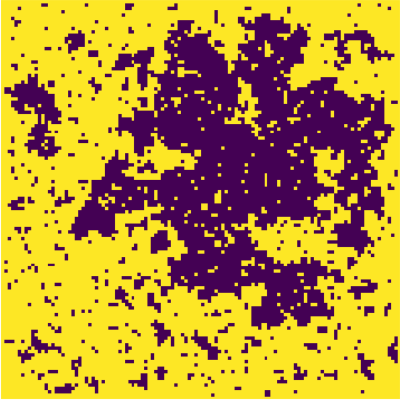
\includegraphics[width=\textwidth]{assets/T2.3-120.pdf}
		\caption{$T= 2.3$}
	\end{subfigure}
	\begin{subfigure}{0.3\textwidth}
		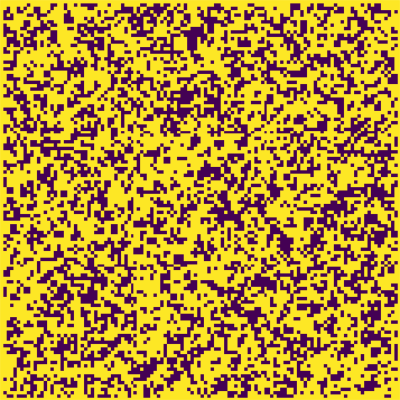
\includegraphics[width=\textwidth]{assets/T6.0-120.pdf}
		\caption{$T= 6.0$}
	\end{subfigure}
	\caption{Configuration probable à $T$ donné -- Phénomène de rupture d'homogénéité}
\end{figure}

\end{frame}


\begin{frame}
\begin{definition}[\'Espérance]
    Soit $f : \Omega_\Lambda \to \mathbf{R}$. L'espérance de $f$ sous $\mu_{\Lambda;\beta}$ est
    \[ \left\langle f \right\rangle_{\Lambda;\beta} \eqdef \sum_{\omega \in \Omega_\Lambda} f(\omega)\mu_{\Lambda;\beta}(\omega)\]
\end{definition}

\begin{itemize}
	\item  Magnétisation spontanée absolue $m \eqdef \left< \left| \sigma_0 \right| \right>_{\Lambda;\beta}$
	\item \'Energie interne $U \eqdef \left< H \right>_{\Lambda;\beta} = - \frac{\partial Z_{\Lambda;\beta}}{\partial \beta}$
	\item Capacité thermique $C \eqdef \frac{\partial U}{\partial T} = k_B\beta^2 \left(\left<E^2\right> -  \left<E\right>^2\right)$
\end{itemize}
\end{frame}

%
\subsection{Résolution naïve}
%

\begin{frame}
		\begin{figure}
			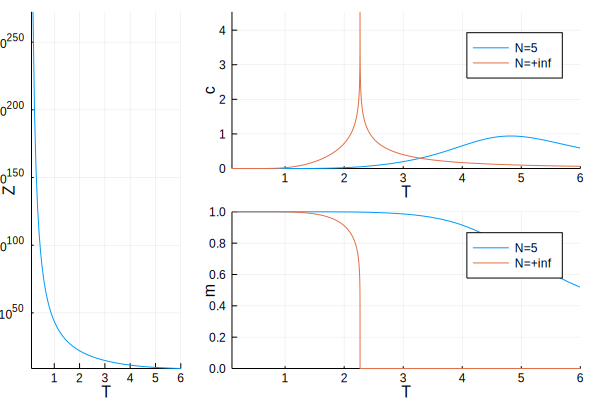
\includegraphics[width=0.7\textwidth]{assets/naif5.pdf}
			\caption{Résolution exacte pour $N=5$ (conditions de bords périodiques) et formule explicite de Lars \bsc{Onsager} pour $N= +\infty$\\$2^{25} \approx 10^7$ configurations, \nombre{3,5} jours de temps de calcul.}
		\end{figure}
	
	
\end{frame}

%
\subsection{Existence d'une transition de phase}
%
\begin{frame}
	\begin{columns}
		\begin{column}{0.4\textwidth}
			\begin{figure}
				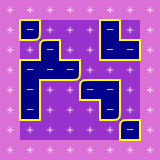
\includegraphics[width=0.9\textwidth]{assets/LTE-small.pdf}
				\caption{Détermination des contours}
			\end{figure}
		\end{column}
		\begin{column}{0.6\textwidth}
			\begin{figure}
				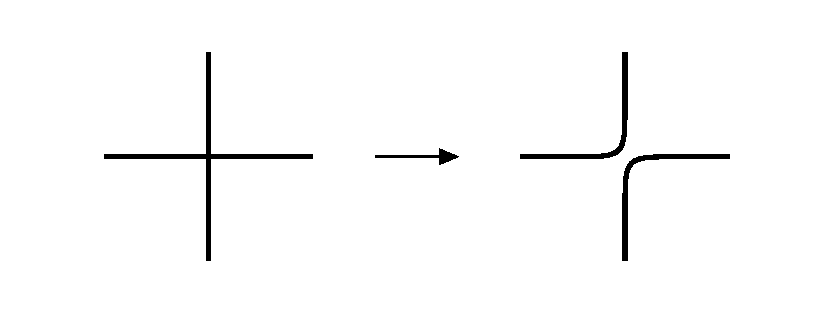
\includegraphics[width=0.6\textwidth]{assets/deformation.pdf}
				\caption{Règle de déformation}
			\end{figure}
			\begin{align*}
				H_\Lambda(\omega) &= -J \left| \mathcal{E}_\Lambda \right| +  2J \sum_{\mathclap{\gamma \in \Gamma(\omega)}} \left| \gamma \right| \\
				\mu_\Lambda\left[\sigma_0 = -1\right] &\leq \mu_\Lambda \left[\exists \tilde{\gamma} \in \Gamma : 0 \in \Int\left(\tilde{\gamma}\right)\right]
			\end{align*}
		\end{column}
	\end{columns}
\end{frame}


%%%
\section{Approche algorithmique}
\subsection{Généralités}
%%%

\begin{frame}
  \begin{itemize}
  	\item \'Echantillonage d'importance
  	\item Dynamique = choix des $R(\omega \to \tilde{\omega})$
  	\item \'Equation maîtresse
  	\begin{align*}
  		\frac{dP_\omega}{dt} = \sum_{\tilde{\omega}} \left[ P_\omega(t)R(\omega \to \tilde{\omega}) - P_{\tilde{\omega}} (t) R(\tilde{\omega} \to \omega)\right]
  	\end{align*}
  	\item Connaissance à priori de $P_\omega$ à l'équilibre :
 	  	\begin{align*}
 	  		P_\omega \xrightarrow[t \to +\infty]{} \mu_{\Lambda;\beta}(\omega)
	  	\end{align*}
  \end{itemize}
\end{frame}

\begin{frame}
\begin{enumerate}[(i)]
	\item Ergodicité : à partir d'une configuration de mesure de Gibbs non nulle, toutes les autres configurations sont atteignables
	\item \'Equilibre détaillé : $P_AW(A \to B) = P_BW(B \to A)$ où $P_A$ est la probabilité d'être dans la configuration $A$ et $W(A \to B)$ est la probabilité de passer de la configuration $A$ à la configuration $B$.
\end{enumerate}
On décompose $W(A \to B) = T(A \to B) \cdot A(A \to B)$ où $T$ est la probabilité que la transition soit proposée et $A$ celle qu'elle soit acceptée.

L'objectif est d'avoir $P_A = \mu(A)$. D'après (ii), cela nous donne 
\begin{align*}
\frac{T(B \to A)\cdot A(B \to A)}{T(A\to B)\cdot A(A \to B)} &= \frac{P_A}{P_B} = e^{-\beta\left(H(A) - H(B)\right)}
\end{align*}
\end{frame}

%
\subsection{L'algorithme Kawasaki}
%

\begin{frame}
	\begin{figure}[htb!]
		\centering
		\begin{subfigure}{0.3\textwidth}
			\centering
			$\begin{matrix}
			\dots & a & d &  \dots \\
			b & s & -s & e\\
			\dots& c & f & \dots
			\end{matrix}$
			\caption{Configuration 1}
		\end{subfigure}
		{\Large $\rightarrow$}
		\begin{subfigure}{0.3\textwidth}
			\centering
			$\begin{matrix}
			\dots & a & d &  \dots \\
			b & -s & s & e\\
			\dots& c & f & \dots
			\end{matrix}$
			\caption{Configuration 2}
		\end{subfigure}
		\caption{Proposition d'échange de spins voisins (en $k$ et $k'$) pour l'algorithme Kawasaki}
	\end{figure}
\begin{align*}
	\Delta H &= -2Js \cdot \left( \sum_{\substack{i \sim k \\ i \neq k'}} \omega_1(i) - \sum_{\substack{i' \sim k' \\ i' \neq k}} \omega_1(i') \right)
\end{align*}
	La transition est acceptée avec une probabilité
	\begin{math}
	\left\{
	\begin{array}{r l}
	0 & \text{si } \Delta{H} \leq 0 \\
	e^{-\beta \Delta{H}} & \text{sinon}
	\end{array}
	\right.
	\end{math}
\end{frame}

%
\subsection{Résultats}
%

\begin{frame}
	\begin{figure}
		\begin{subfigure}{0.3\textwidth}
			
\includegraphics[width=\textwidth]{assets/T0.1-120.pdf}
			\caption{$T= 0.1$}
		\end{subfigure}
		\begin{subfigure}{0.3\textwidth}
			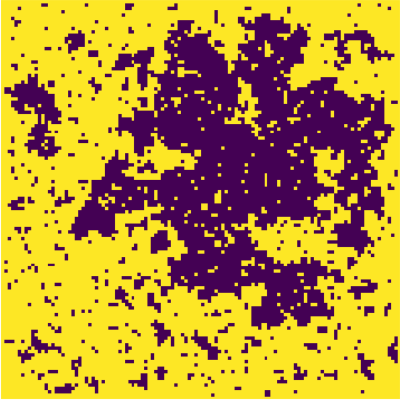
\includegraphics[width=\textwidth]{assets/T2.3-120.pdf}
			\caption{$T= 2.3$}
		\end{subfigure}
		\begin{subfigure}{0.3\textwidth}
			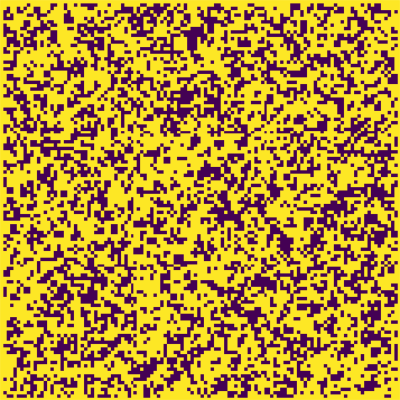
\includegraphics[width=\textwidth]{assets/T6.0-120.pdf}
			\caption{$T= 6.0$}
		\end{subfigure}
\caption{Modélisation numérique : système après \nombre{600000} balayages\\(1 balayage = $N^2$ propositions d'échange ; $N =120$)}
	\end{figure}

\end{frame}

\begin{frame}
\begin{figure}
	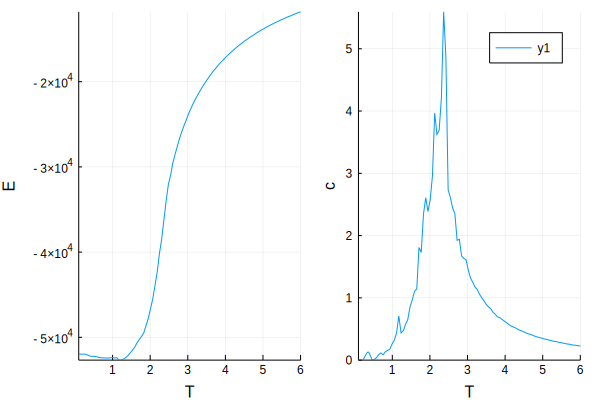
\includegraphics[width=0.8\textwidth]{assets/mesures120.pdf}
	\caption{Modélisation numérique : système après \nombre{600000} balayages\\(1 balayage = $N^2$ propositions d'échange ; $N =120$)}
\end{figure}

\end{frame}

\section{Annexe}
\subsection*{Annexe}
\bgroup
\setbeamercolor{background canvas}{bg=gray}
\begin{frame}[plain]{}
\end{frame}
\egroup

\subsection*{En une dimension}


\begin{frame}
\begin{figure}
	\centering
	\begin{tikzpicture}
	%\fill[blue!40!white] (-4,0) rectangle (-3,1);
	%\fill[blue!40!white] (3,0) rectangle (4,1);
	\draw[step=1cm,color=gray] (-4,0) grid (4,1);
	\node at (-3.5,+0.5) {$+1$};
	\node at (-2.5,+0.5) {$-1$};
	\node at (-1.5,+0.5) {$+1$};
	\node at (-0.5,+0.5) {$-1$};
	\node at (0.5,+0.5) {$-1$};
	\node at (1.5,+0.5) {$+1$};
	\node at (2.5,+0.5) {$-1$};
	\node at (3.5,+0.5) {$-1$};
	\end{tikzpicture}
	\caption{Une configuration $\sigma$ avec condition de bords périodique, $N = 6$}
\end{figure}
En une dimension, sur un graphe de longueur $N$ soumis à un champ $h$, le Hamiltonien avec condition aux bords  périodique (dans l'ensemble grand canonique) devient
\begin{align*}
H(\sigma) &= -J \sum_{i = 1}^{N} \sigma(i) \sigma(i + 1) -h \sum_{i = 1}^{N} \sigma(i) \\
& = -J \sum_{i = 1}^{N} \sigma(i) \sigma(i + 1) -\frac{h}{2} \sum_{i = 1}^{N} \left[\sigma(i) + \sigma(i+1)\right]\\
\end{align*}
\end{frame}

\begin{frame}
\begin{align*}
e^{-\beta H(\sigma)} &= \prod_{i = 1}^{N} e^{\beta \left(J\sigma(i)\sigma(i+1) +\frac{h}{2}\left(\sigma(i) + \sigma(i+1)\right)\right) }
\end{align*}
On pose la matrice de transfert
\[T =
\begin{pmatrix}
T_{++} & T_{+-} \\
T_{-+}  &  T_{--}
\end{pmatrix}
=
\begin{pmatrix}
e^{\beta(J + h)}  &   e^{\beta(- J)} \\
e^{\beta(-J)} & e^{\beta(J - h)}
\end{pmatrix}
\]
On a alors
\begin{align*}
e^{-\beta H(\sigma)} =& \prod_{i}^{N} T_{\sigma(i), \sigma(i+1)}
\end{align*}
\end{frame}

\begin{frame}
Calculons la fonction de partition :
\begin{align*}
Z_\beta &\eqdef \sum_{\sigma \in \left\{-1, +1\right\}^N} e^{-\beta H(\sigma)} \\
&=\sum_{\sigma(0) = \pm 1} \dots \sum_{\sigma(N) = \pm 1} \prod_{i}^{N} T_{\sigma(i), \sigma(i+1)} \\
&= \Tr\left(T^N\right)
\end{align*}
\end{frame}

\begin{frame}

\begin{align*}
T =
\begin{pmatrix}
e^{\beta(J + h)}  &   e^{\beta(- J)} \\
e^{\beta(-J)} & e^{\beta(J - h)}
\end{pmatrix}
\in S_2\left(\mathbf{R}\right)
\end{align*}
est orthogonalement diagonalisable (Th. spectral), notons \(\Sp\left(T\right) = \left\{\lambda_+, \lambda_-\right\}\).
\begin{align*}
\chi_T &= X^2 - \left(e^{\beta(J + h)} + e^{\beta(J - h)}\right) + e^{2\beta J} - e^{-2\beta J} \\
& = X^2 - e^{\beta J}  2\cosh(\beta h) + 2\sinh(2\beta J)\\
\lambda_\pm &= \frac{2e^{\beta J}\cosh(\beta h) \pm \sqrt{4e^{2\beta J}\cosh^2(\beta h) + 8\sinh(2\beta J)}}{2} \\
&= e^{\beta J}\cosh(\beta h) \pm \sqrt{e^{2\beta J}\cosh^2(\beta h) + 2\sinh(2\beta J)}
\end{align*}

\end{frame}


\begin{frame}
\begin{align*}
Z_\beta &= \Tr\left(T^N\right) = \lambda_+^N + \lambda_-^N\\
f_N(\beta,h) &= \frac{1}{N} \log\left(Z_{\beta,N}\right) \\
&=  \log\left(\lambda_+\right)  + \log\left(1 + \left(\frac{\lambda_-}{\lambda_+}\right)^N \right)
\end{align*}
Or, $0 \leq \lambda_- < \lambda_+$. On conclut
\begin{align*}
f(\beta, h) &= \log\left(\lambda_+\right) \\
&= \log\left( e^{\beta J}\cosh(\beta h) \pm \sqrt{e^{2\beta J}\cosh^2(\beta h) + 2\sinh(2\beta J)} \right)
\end{align*}
\end{frame}


\begin{frame}
\begin{columns}[c]
\column{.3\textwidth}
On définit l'énergie libre
\begin{align*}
f = - \frac{\ln Z_\beta}{N \beta}
\end{align*}
\column{.7\textwidth}
\vspace*{-1.5cm}
\begin{figure}
\centering
\includegraphics[height=0.65\textheight]{assets/Elibre}
\caption{\'Energie libre par n\oe{}ud en fonction de $T$}
\label{fig:elibre}
\end{figure}
\end{columns}
\end{frame}


    %\nocite{*}
    %\printbibliography
\end{document}
